\documentclass[11pt, letterpaper]{article}  % change to >11 pt if you like, and change article with report
\usepackage[letterpaper, top=3.71cm, bottom=3.20cm, left=2.86cm, right=2.86cm]{geometry}
\usepackage[utf8]{inputenc}
\usepackage{natbib}
\usepackage{graphicx}
\usepackage{color}
\usepackage{subfig}
\usepackage{float}
\usepackage{hyperref}
\usepackage{url}
\usepackage{minted}
%\usepackage{algorithmic}
%\usepackage{algpseudocode}
\usepackage[linesnumbered,ruled,vlined]{algorithm2e}
\usepackage[table, dvipsnames]{xcolor}
\usepackage{multirow}
\usepackage{wrapfig}
\newcommand{\dash}{{-}}%

\title{\vspace{-2cm}\textbf{Parallel and Distributed Systems project report\\K-Nearest Neighbours}}
\author{\textbf{\small{\textit{Ristori Alessandro}}} \\ % put your full name here
        \small{Master Degree in Computer science.}\\ \small{{a.ristori5@studenti.unipi.it, 619618}} \\  % put your Master Degree here
        \small{Parallel and Distributed Systems, Academic Year: 2020/2021} \\
        \small{Date: 3/02/2022} \\
       %\textbf{\small{\url{https://github.com/RistoAle97/PDS}}}
}

\renewcommand\refname{} %remove this line to automatically show the bibliography header

\begin{document}
\nocite{*}  % comment this line to list only the articles you really cite
\date{}
\maketitle
\begin{center}
    
\includegraphics[width=0.45\textwidth]{images/unipi.png}\\
    \vspace{0.5cm}
\end{center}
\thispagestyle{empty}
\newpage
%\thispagestyle{empty}
\tableofcontents
\thispagestyle{empty}
\newpage
%\listoffigures
%\newpage
\pagenumbering{arabic}
\section{Introduction}\label{sec:introduction}
The K-Nearest Neighbours is a well known classification method used to classify datapoints given their spatial representation without the complexity of models such Neural Networks. A point is classified in a determined class by a majority vote of its \textit{k} neighbours, where \textit{k} is an hyperparameter and the only one that KNN needs.
\vspace{3mm}

The aim of the project was not a classification task or to learn the best value of \textit{k}, but to find the nearest \textit{k} neighbours for all the points in a 2d space and writing the results into another file. The input dataset is composed by pairs of coordinates which represents the points, the output file contains an ordered list for each point with their \textit{k} nearest neighbours ordered by distance. Moreover, the main purpose of the project was to find a way to parallelize this modified version of KNN with both C++ standard library threads and FastFlow library.
\section{Implementation}
In this section I'll discuss of the main implementation choices taken during the development of the project by also giving an overview on the method itself.

\subsection{KNN overview}\label{subsec:knn_overview}
Before we dive into the heart of the section we need to contestualize KNN inside the project. KNN is a perfect example of \textbf{Data Parallel problem} and, more precisely, an \textbf{embarassingly parallel} one, because the \textbf{computation of a subtask is independent to the others}, therefore those subtasks don't need any kind of communication or synchronization.
The task can be summarized as the composition of three major steps:
\begin{itemize}
    \item \textbf{Read all the points} on a 2d space from a file.
    \item\textbf{Compute KNN}.
    \item \textbf{Write results} on file.
\end{itemize}
Without a doubt the most computationally expensive and interesting part is the second one, which I will talk more about on \autoref{subsec:seq_implementation}.

\subsection{Sequential implementation}\label{subsec:seq_implementation}
As I said at the end of \autoref{sec:introduction}, the project required two different versions of the same task, one using C++ threads from stdlib and one using FastFlow, but both share the same main structure and, therefore, I thought that it would be useful to show it in \autoref{algorithm:knn} (which is the sequential version of KNN method) in order to better understand how it works.

\SetKwInput{KwInput}{Input}
\SetKwInput{KwOutput}{Output} 
\begin{algorithm}[H]
    \caption{KNN sequential}
    \label{algorithm:knn}
    \KwInput{txt file containing a pair of coordinates for each row representing the points, the index of a point is the row on which such pair is located and the value of k}
    \KwOutput{string which will be written on a file where the i-th row is in the following format: $point_{i}: <neigh\_id_{1}, distance_{i1}>, ... <neigh\_id_{n}, distance_{in}>$}
    \textbf{Read points} from file and store them into \textit{points}\\
    \textbf{Priority queue} knn\\
    \textbf{String} knn\_results\\
    \For{point i in points} {
        \For{points j in points} {
            \If{$i==j$} {
                continue
            }
            calculate \textit{d(i, j)}\\
            \If{$knn.size()<k$} {
                knn.emplace(point[j])
            }\ElseIf{$d(i,j)<knn.top()$} {
                knn.pop()\\
                knn.emplace(point[j])
            }
        }
        \While{$!knn.empty()$} {
            p = knn.pop()\\
            knn\_results.append(to\_string(p))
        }
    }
    \textbf{Write knn\_results} to file
\end{algorithm}
The main choice was to \textbf{keep a single priority queue globally} with \textit{k} as its dimension, which is emptied at the end of the first inner loop in order to write the results in the final output string, this is surely better than keeping as much priority queues as the number of points, which would have been a serious waste of space the more the latter went up.
\vspace{3mm}

Moreover, the priority queue was preferred since it can retrieve istantly (i.e.: with constant cost) the most distant point in the structure so the only thing that has a notable cost is the reestablishment of the priority condition which is $O(log(k))$, way better than $O(klog(k))$ that would have taken by ordering a normal array of \textit{k} points.
\vspace{3mm}

\subsubsection{Sequential cost}
The total cost of the first inner loop is given by the cost of computing distances, $O(n)$, and the cost to mantain the priority condition for a complexity of $O(nlog(k))$, this part of the method will be known as \textit{knn} and its completion time will be $T_{knn}$ from now on; at the same time, the building of the ouptut string has cost $O(klog(k))$ and its completion time will be known as $T_{BuildString}$, so the final cost of the KNN computation is:
\begin{center}
\begin{Large}
$O(n(nlog(k)+klog(k)))=O(n^2log(k)+nklog(k))=O(n^2log(k))$
\end{Large}
\end{center}

The previous statement holds always true if $k<<n$, which is the case of this project; we can now define the completion time of the sequential version as:

\begin{center}
\begin{Large}
$T_{seq}=T_{Read}+n(T_{knn}+T_{BuildString})+T_{Write}$
\end{Large}
\end{center}
where $n$ is the number of points, $T_{knn}$ is the time spent on finding the \textit{k} closest points and $T_{BuildString}$ is the time spent to build the output string. $T_{Read}$ and $T_{Write}$ are autoexplicative and they represent the \textbf{serial part} of the source code.

\subsection{Parallel implementations}\label{subsec:par_implementations}
As required from the project, I developed two more implementations of KNN, one using C++ threads and the other using the FastFlow library.
\subsubsection{C++ threads}
The parallel implementation with threads from the standard library of C++ is straightforward since it is nearly the same as the sequential one with some tweaks. Each thread has assigned the same number of points in an extremely easy way, given $nw$ as the number of workers. the \textbf{workload} is defined as $\frac{n}{nw}$ and the \textbf{excess amount of work} as $n\%nw$ which needs to be redistributed between the threads, so at maximum we need to redistribute $nw-1$ of excess workload and, since $nw<<n$, this is highly negligible with respect to the KNN computation.
\vspace{3mm}

\textbf{Each thread knows where its partition starts and ends} given its workload and id, therefore the threads work on their partition at the same time just like a \textit{Map} template.
Moreover, \textbf{each thread returns a string} (just like for the sequential implementation) which is saved in an array in position $i$ that corresponds to the thread id and at the end the results are written on the output file by combining one string at time, like in a \textit{Reduce} fashion.
\vspace{3mm}

The only cons from this implementation come from the \textbf{increased number of priority queues}, which is now the same as the number of threads, and the \textbf{overhead cost} since we need to split and merge the work.

\subsubsection{FastFlow}
\textbf{The fastflow implementation is nearly identical to the C++ threads one} and even simpler since I did not need to load balance the workload manually. I opted to use a \textbf{ParallelForReduce} since it works in the same way as I did for the stdlib threads version (i.e.: a Map followed by a Reduce, keep in mind that in this way the Map's collector is substituted by the Reduce).

\subsubsection{Parallel cost}
\textbf{Both C++ threads and FastFlow implementations rely on \autoref{algorithm:knn}}, so their cost is similar but, since the outer loop can be done in parallel now, the weight of the main argument that contributes the most (i.e.: $n(T_{knn}+T_{BuildString})$ is now divided by the number of workers.
\vspace{3mm}

Even though the weight of the most expensive part is alleviated, \textbf{the cost coming from the task subdivision and final merge should be taken into account as pure overhead} $T_{ov}=T_{Split}+T_{Reduce}$. Hence, the total cost of the parallel implementations can be defined as:

\begin{center}
\begin{Large}
$T_{par}(nw)=T_{Read}+nwT_{ov}+\frac{n(T_{knn}+T_{BuildString})}{nw}+T_{Write}$
\end{Large}
\end{center}
Where $nw$ is the number of workers or, more technically speaking, the \textbf{parallelism degree} and everything else was the same as discussed during the sequential version.
\section{Results}
This section will show what kind of setup was used to test the performances of our implementations and what results were achieved.

\subsection{Expected results}
First of all\textbf{ I expected the completion times of both implementations to be somewhat similar} given their same structure, this implies that they will also have some \textbf{similarity on their speedup and others metrics}.
\vspace{3mm}

Speaking about the speedup, we know that it is equal to $\frac{T_{seq}}{T_{par(nw)}}$ and that the ideal one is exactly the parallelism degree, $nw$; this means that, in a real world environment, the achievable speedup is $s(nw)<nw$, let's check it this fact holds:
\begin{center}
\begin{Large}
$s(nw)=\frac{T_{seq}}{T_{par}}=\frac{T_{Read}+n(T_{knn}+T_{BuildString})+T_{Write}}{T_{Read}+nwT_{ov}+\frac{n(T_{knn}+T_{BuildString})}{nw}+T_{Write}}$
\end{Large}
\end{center}
It is safe to assume that $T_{Read}$ and $T_{Write}$ are negligible with respect to the total completion time so everything reduces to:
\begin{center}
\begin{Large}
$s(nw)=\frac{n(T_{knn}+T_{BuildString})}{nwT_{ov}+\frac{n(T_{knn}+T_{BuildString})}{nw}}$
\end{Large}
\end{center}
And this is surely less than $nw$ as we know from the lectures.

\subsection{Setup}
Before we talk about the results I decided that it was necessary to explain some choices beforehand:
\begin{itemize}
    \item The results were all obtained on the \textbf{64-core with four-way hyperthreading Intel XEON-PHI}.
    \item For each configuration \textbf{I did not take into consideration $T_{Read}$, $T_{Write}$ and $T_{ov}$} since they were nearly the same for each configuration with the same amount of points, moreover the most interesting part is the \textit{non-serial} one, which is $n(T_{knn}+T_{BuildString})$.
    \item \textbf{Each configuration was run ten times}.
    \item The\textbf{ chosen value for k was 10 for all the configuration}, hence all the results in the next subsections are averages.
    \item The \textbf{parallelism degree was decided to be $2^i$} where $i\in\{0, .., 8\}$.
    \item \textbf{Times were obtained using the utimer class} that the professor showed during the lectures.
\end{itemize}
\subsection{Results on the XEON-PHI machine}
I decided to run tests on 2d spaces with \textbf{10k, 20k, 50k and 100k points} where every point was drawn by an uniform distribution over [0, 10]; the number of points was decided as such in order to see \textbf{how each implementation perform going from a sparse spaces to densely populated ones}. First of all it was necessary to calculate the amount of time spent by the execution of the sequential knn version in order to get values needed to obtain the other metrics (e.g.: speedup and efficiency), \autoref{table:knn_sequential_results} shows the results achieved by such implementation.

\begin{table}[H]
\centering
\begin{tabular}{c|c|c|c}\hline \hline
\multicolumn{4}{c}{\textbf{Sequential 10-KNN execution times ($\mu$sec)}} \\\hline
\textbf{10k points} & \textbf{20k points} & \textbf{50k points} & \textbf{100k points}\\\hline
4187051 & 15973321 & 95360616 & 375058248 \\
\hline \hline
\end{tabular}
\caption{Results with the sequential implementation.}
\label{table:knn_sequential_results}
\end{table}
As one would expect, the time does not scale linearly with the number of points since the cost of \autoref{algorithm:knn} is $O(n^2log(k))$, something more interesting arose during the execution of C++ threads and FastFlow versions whose results are shown in \autoref{table:knn_parallel_fastflow_results}.

\begin{table}[H]
\centering
\begin{tabular}{c||c|c|c|c||c|c|c|c}\hline \hline
\multicolumn{9}{c}{\textbf{Parallel and FastFlow 10-KNN execution times ($\mu$sec)}} \\\hline \hline
\multirow{2}{*}{\textbf{nw}} & \multicolumn{4}{c||}{\textbf{stdlib threads}} & \multicolumn{4}{c}{\textbf{FastFlow}} \\\cline{2-9}
& \textbf{10k} & \textbf{20k} & \textbf{50k} & \textbf{100k} & \textbf{10k} & \textbf{20k} & \textbf{50k} & \textbf{100k} \\\hline
1 & 4195076 & 16573213 & 98816008 & 377017508 & 4198343 & 15989082 & 96277045 & 406293436 \\
2 & 2150114 & 8006220 & 50251728 & 201949754 & 2124308 & 8018496 & 48329593 & 201459406 \\
4 & 1324868 & 4072286 & 27676599 & 99481003 & 1072248 & 4034389 & 2422181 & 99968804 \\
8 & 726914 & 2030168 & 13578018 & 51113708 & 539050 & 2021035 & 12098202 & 50136748 \\
16 & 322046 & 1087086 & 6741971 & 24312895 & 316082 & 1062674 & 6183317 & 26882276 \\
32 & 182296 & 677542 & 3472759 & 14382776 & 210621 & 588005 & 3461644 & 14591443 \\
64 & 133958 & 434134 & 2151317 & 8876960 & 141363 & 400733 & 2278688 & 9016368 \\
128 & 99786 & 308973 & 1590471 & 6123643 & 106730 & 318886 & 1665072 & 6326216 \\
256 & 99371 & 256716 & 1046949 & 3969818 & 95743 & 274393 & 1122244 & 4312146 \\ \hline \hline
\end{tabular}
\caption{Results with the stdlib threads and FastFlow implementations.}
\label{table:knn_parallel_fastflow_results}
\end{table}

\subsection{Results analysis}
As first thing I want to underline is the fact that \textbf{the results are extremely similar between the two implementations} since, as I said in \autoref{subsec:par_implementations}, the two versions are basically the same with some minor changes.

\subsubsection{Execution times}
The execution times comparison (only for 50k and 100k points) is shown in \autoref{fig:results}
\begin{figure}[H]
    \centering
    \subfloat[C++ threads]{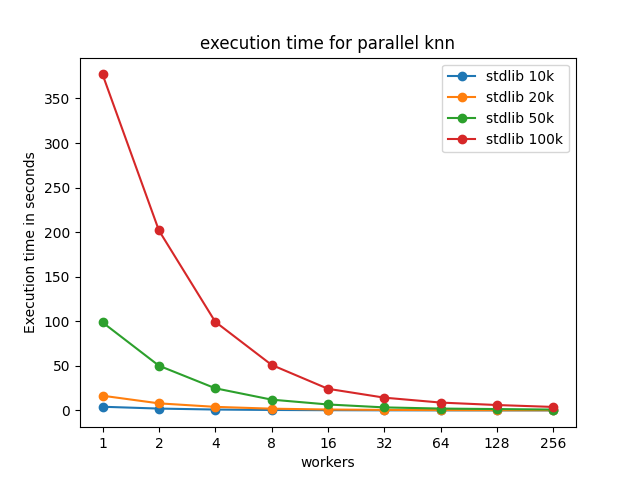
\includegraphics[width=0.45\linewidth]{images/knn_parallel_results.png}}
    \subfloat[FastFlow]{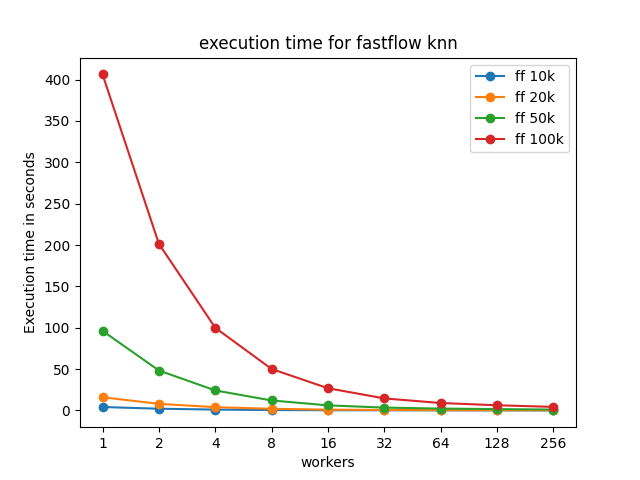
\includegraphics[width=0.45\linewidth]{images/knn_fastflow_results.png}}\\
    \subfloat[Comparison]{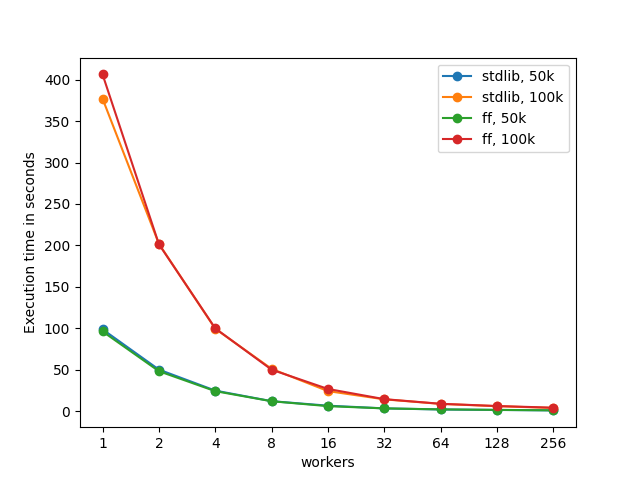
\includegraphics[width=0.45\linewidth]{images/knn_comparison_results.png}}
    \caption{Execution times for C++ threads and FastFlow versions and their comparison}
    \label{fig:results}
\end{figure}

\subsubsection{Speedup}
Let's now see and compare the speedup obtained by both implementations as shown in \autoref{fig:speedup}
\begin{figure}[H]
    \centering
    \subfloat[C++ threads]{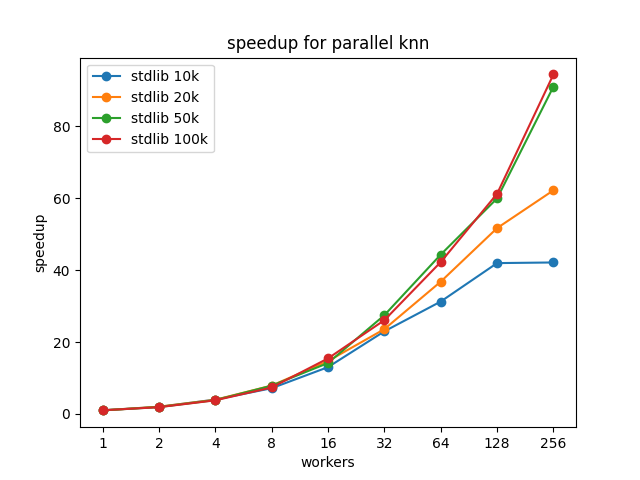
\includegraphics[width=0.45\linewidth]{images/knn_parallel_speedup.png}}
    \subfloat[FastFlow]{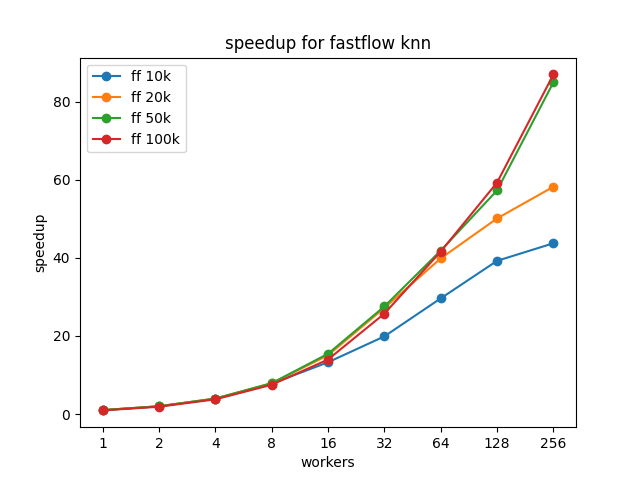
\includegraphics[width=0.45\linewidth]{images/knn_fastflow_speedup.png}}\\
    \subfloat[Comparison]{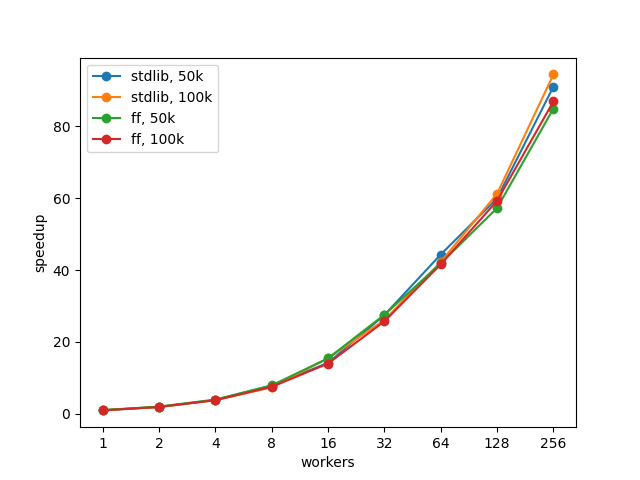
\includegraphics[width=0.45\linewidth]{images/knn_comparison_speedup.png}}
    \caption{Speedup for C++ threads and FastFlow versions and their comparison}
    \label{fig:speedup}
\end{figure}
The \textbf{speedup seems to scale well with the number of workers as long the number of points goes up}, in fact I could clearly see that for sparse 2d spaces (e.g.: 10k and 20k points) \textbf{the speedup seemed to reach a sort of plateau} the more I increased $nw$.
\vspace{3mm}

Since the execution times are the same \textbf{it was natural that the two versions would have similar speedup}, this will be the same for the next metrics that we are going to see.
\subsubsection{Scalability}
Scalability is the ratio between the parallel execution time with parallelism degree equal to 1 and the parallel execution with parallelism degree equal to $nw$, the ideal value is the same as for the speedup ($nw$).
\begin{center}
\begin{Large}
$scalab(nw)=\frac{T_{par}(1)}{T_{par(nw)}}$
\end{Large}
\end{center}
It measures how the parallel implementation achieves efficiently better performance the more the parallelism degree increases.
\begin{figure}[H]
    \centering
    \subfloat[C++ threads]{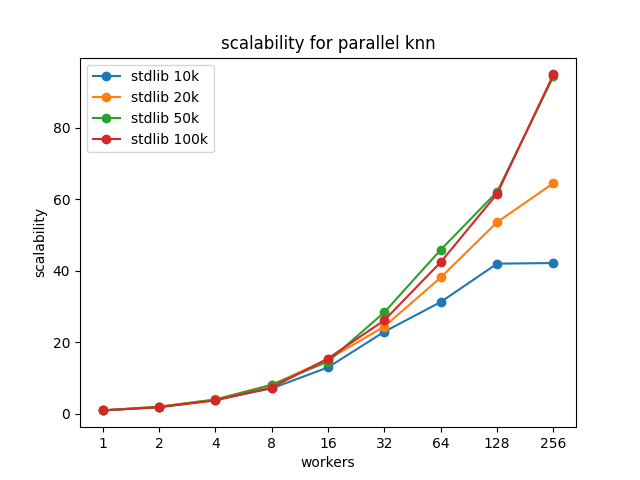
\includegraphics[width=0.45\linewidth]{images/knn_parallel_scalability.png}}
    \subfloat[FastFlow]{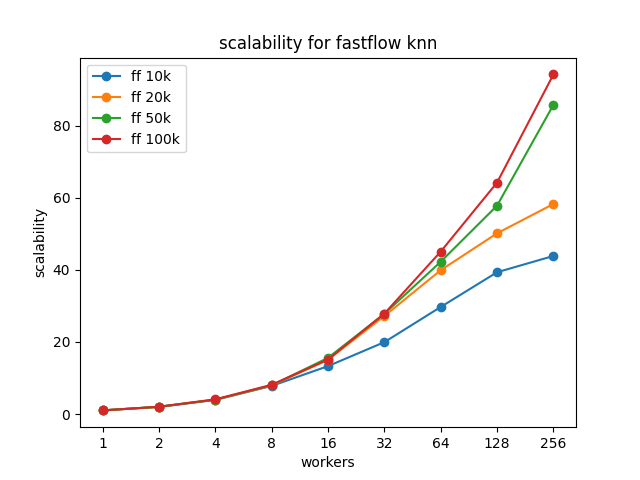
\includegraphics[width=0.45\linewidth]{images/knn_fastflow_scalability.png}}\\
    \subfloat[Comparison]{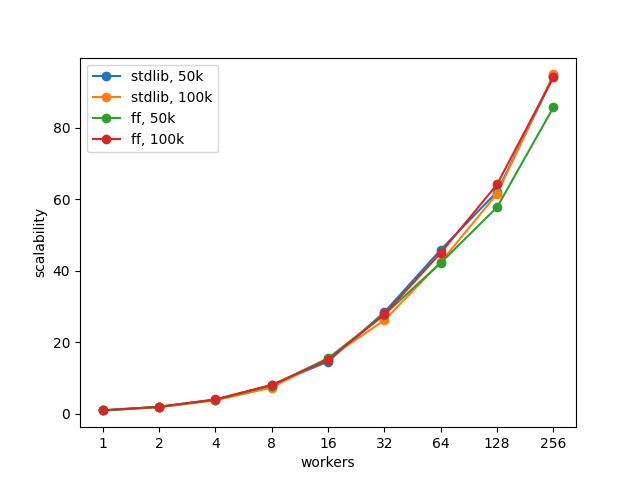
\includegraphics[width=0.45\linewidth]{images/knn_comparison_scalability.png}}
    \caption{Scalability for C++ threads and FastFlow versions and their comparison}
    \label{fig:scalability}
\end{figure}
What we have discussed briefly during the speedup analysis holds for the scalability too.

\subsubsection{Efficiency}
As last metric of the analysis it was natural to choose efficiency which is the ratio between the ideal execution time and the actual execution time.
\begin{center}
\begin{Large}
$\epsilon(nw)=\frac{T_{id}(nw)}{T_{par}(nw)}=\frac{T_{seq}}{nwT_{par}(nw)}=\frac{s(nw)}{nw}$
\end{Large}
\end{center}
The formula holds since $T_{id}=\frac{T_{seq}}{nw}$, moreover \textbf{efficiency measures how a parallel implementation is making use of the available resources}. The ideal value for the efficiency is 1 given the fact that the speedup is bound by $nw$.
\begin{figure}[H]
    \centering
    \subfloat[C++ threads]{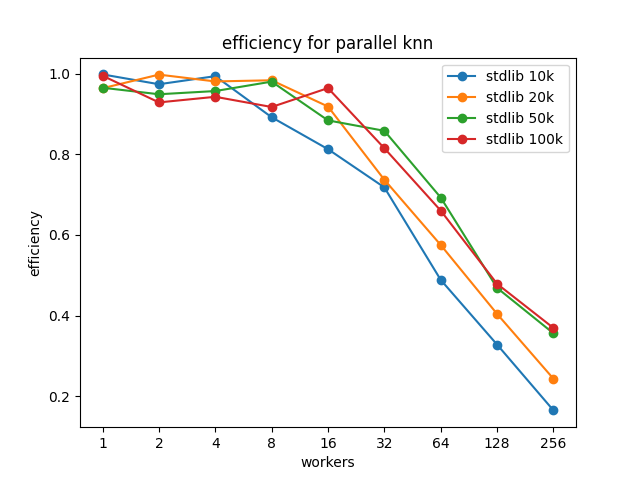
\includegraphics[width=0.45\linewidth]{images/knn_parallel_efficiency.png}}
    \subfloat[FastFlow]{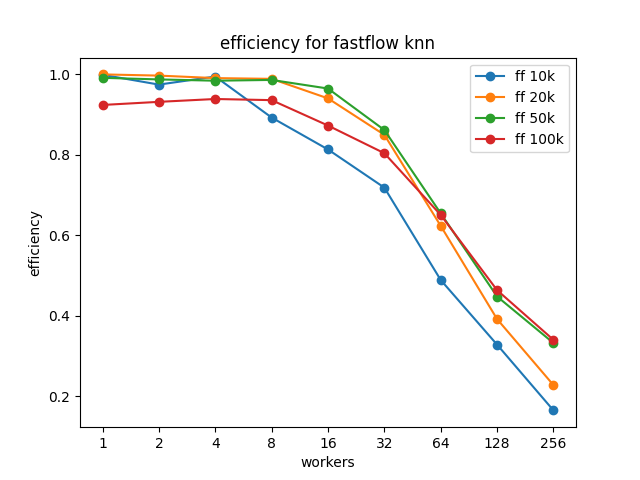
\includegraphics[width=0.45\linewidth]{images/knn_fastflow_efficiency.png}}\\
    \subfloat[Comparison]{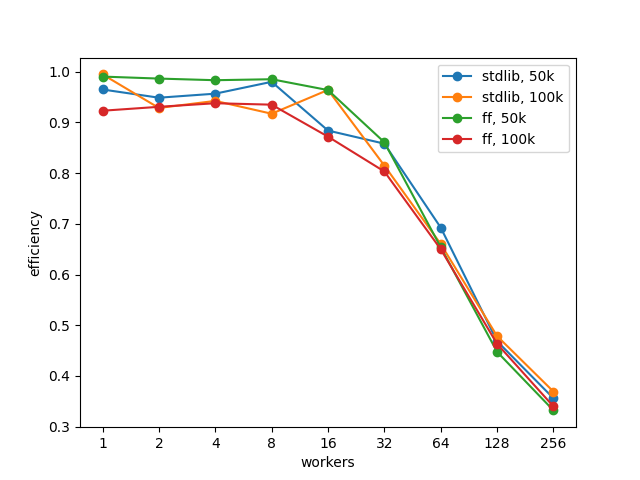
\includegraphics[width=0.45\linewidth]{images/knn_comparison_efficiency.png}}
    \caption{Efficiency for C++ threads and FastFlow versions and their comparison}
    \label{fig:efficiency}
\end{figure}
The most interesting thing is the fact that the efficiency has a strange plot from 2 to 16 workers as shown in \autoref{fig:efficiency}, this could be caused by the congestion on the XEON-PHI machine from other students while I was working on it (but I do not want to blame them as everyone needs to do project) or by routine tasks of the machine itself.
\vspace{3mm}

Another thing is the fact that \textbf{configurations with more points had a better efficiency than the ones working on sparse spaces}, but this comes to no surprise since the former had an higher speedup than the latter.
\section{Improvements}
Meanwhile I was working on the project many other solutions or improvements came to my mind that at the end were not implemented for various reasons, in this subsection i will explain some of them.
\vspace{3mm}

\subsection{Parallelize everything}
First, is possibile to parallelize both the outer loop and first inner loop from \autoref{algorithm:knn}, however this comes with the price that the threads working on the inner loop have to insert or remove points from the priority queue by "communicating" with the others, this implies an higher overhead.
I could also parallelize the reading and writing part but since their cost was small with respect to the KNN computation I thought that it would not have any major improvement.
\vspace{3mm}

\subsection{Compute more efficiently the distances}
Then it is possible to compute the distances by calculating the upper or lower triangular distance matrix, but even this solution comes with an higher overhead since a thread would need to access two priority queues at the same time (for two different points i and j) and one of them could be accessed at the same instant by another thread (this is the same "communication" problem as before). Moreover the computation of the distances in this way has the same cost of my solution, $O(n^2)$, so it was discarded right away.
\vspace{3mm}

\section{Running the project}
To build everything needed to test the project you can make use of the Makefile just by typing \textit{make} once you have extracted the zip file.
\vspace{3mm}

Afterwards, you can generate datasets of points with \textit{generate\_points.py} using it in the following way (it will create 10000 points by using a uniform distribution between 0 and 10 if no arguments are passed):
\begin{minted}[fontsize=\small, bgcolor=gray!30]{bash}
python generate_points.py --n 100000 --file datasets/points.txt
\end{minted}

Then you can run every implementation easily, the following are just examples:
\begin{minted}[fontsize=\small, bgcolor=gray!30]{bash}
./knn_sequential datasets/points.txt 10
./knn_parallel datasets/points.txt 10 256
./knn_ff datasets/points.txt 10 256
\end{minted}

For each implementation the second argument is the value of k, meanwhile the third argument, for both stdlib threads and FastFlow implementations, is the number of workers.
If you want to execute more times the same implementation or to execute more than one at time, use the \textit{compute\_knn.py} method:
\begin{minted}[fontsize=\small, bgcolor=gray!30]{bash}
python --file datasets/points_10k.txt --k 10 --nw 256 --runs 10 --execute spf
\end{minted}
The last argument specifies what versions to run (s for sequential, p for parallel and f for FastFlow).
\include{chapters/references}
\end{document}
